\section{Model Evaluation}
\label{sec:Model-Evaluation}
\index{PerfModel!Model Evaluation}

This section introduces the experiments with our simulator to show when reactive load balancing can be late sometimes, leading to late decisions in offloading tasks. Our evaluation metric for this case is the decrease in queue length. Each process, in general, has a global queue of tasks. The execution threads per process get tasks from the queue for execution. Therefore, the queue length will be decreased toward $0$ over time steps, where the slowest process with queue length converging to $0$ determines the completion time of our application.\\

To be again consistent with the addressed example in the previous sections, we configure the simulation with $8$ ranks. Each rank here keeps $100$ tasks\footnote{To get the simulation results faster, we have reduced the number of tasks to $100$, compared to the one of $1000$ tasks in Figure \ref{fig:react_lb_simulation_1000_tasks_per_rank_example}.} at the beginning. Two of $8$ ranks are $5\times$ slower than normal, and the normal execution rate is $1$ tasks/second. This means the two slowdown ranks take $5$s to complete a task, while the others take $1$s for a task. In case of no load balancing, the completion time is $500$s because the two bottleneck ranks take $5$s/task. $R_{imb}$ is about $1.5$, clock timing is counted in one-by-one step, in which each step is $1$ms. Alongside, there are two variables varied in the experiments:
\begin{itemize}
	\item Balancing overhead ($O_{\text{balancing}}$): the values are varied such as $1, 2, 5, ...$, accounting for $0.1\%$, $0.2\%$, $0.5\%$ of overhead. 
	\item Delay time in task migration ($d$): its values are also varied such as $1, 2, 5, ...$, and also accounting for $0.1\%$, $0.2\%$, $0.5\%$ of overhead. 
\end{itemize}

\noindent \textbf{Vary delay ($d$) and keep balancing overhead ($O_{\text{balancing}}$) stable}\\
\noindent In this set of simulations, we vary the values of $d$ in a range of $[$ $0.1\%$, $0.2\%$, $0.5\%$, $1\%$, $2\%$ $]$, and keep the values of $O_{\text{balancing}}$ as a constant. \\

\begin{figure}[t]
  \centering
  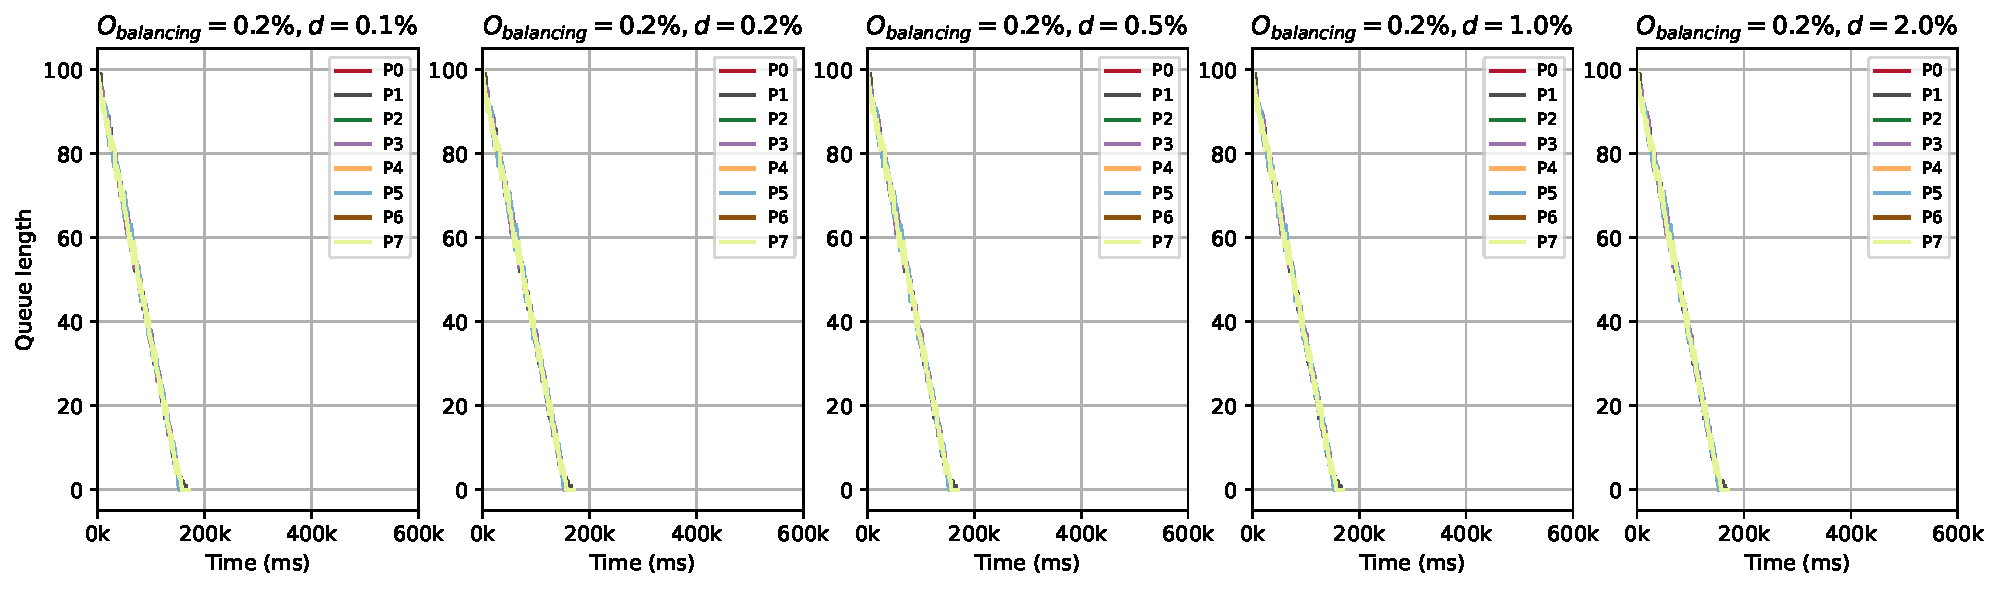
\includegraphics[scale=0.45]{./pictures/perf_analysis_model/perf_model_queue_decrease_delay_impact_OB2.pdf}
	\caption{A simulation case to show the impact of delay time ($d$) with keeping the overhead of balancing operations as a constant of $0.2\%$.}
	\label{fig:react_lb_sim_delay_impact_Obal_2}
\end{figure}

Figure \ref{fig:react_lb_sim_delay_impact_Obal_2} shows a simulation experiment with the varied values of delay ($d$), while we keep the value of balancing overhead as a constant of $0.2\%$. Note that the percentage means the ratio with task runtime unit. Here the runtime is in seconds, and the values of $d$ or $O_{\text{balancing}}$ are in milliseconds. Therefore, $O_{\text{balancing}}$, in this case, takes $2$ms, occupying $0.2\%$ of a task runtime unit. As the figure shows, there are $8$ processes, where each line indicates the decrease or the convergence of its queue to $0$ over the execution time progress (on the x-axis). The y-axis shows the queue length values. At the very beginning, the queue length of all processes is the same, $100$ tasks. Following execution and reactive load balancing, they tend to decrease steadily but might sometimes increase if receiving tasks from a remote process. There are five plots from left to right, illustrating the simulation when $d$ is varied from $0.1\%$ to $2\%$. The time that the last process goes to $0$ also highlights the completion time. Figure \ref{fig:react_lb_sim_delay_impact_Obal_2} shows that the increasing values of $d$ do not highly change the completion time in this case. Such a baseline, if we do not apply any load balancing methods, the completion time will be $500k$. Therefore, the simulating case in Figure \ref{fig:react_lb_sim_delay_impact_Obal_2} shows that reactive load balancing is significantly useful.\\

\begin{figure}[t]
  \centering
  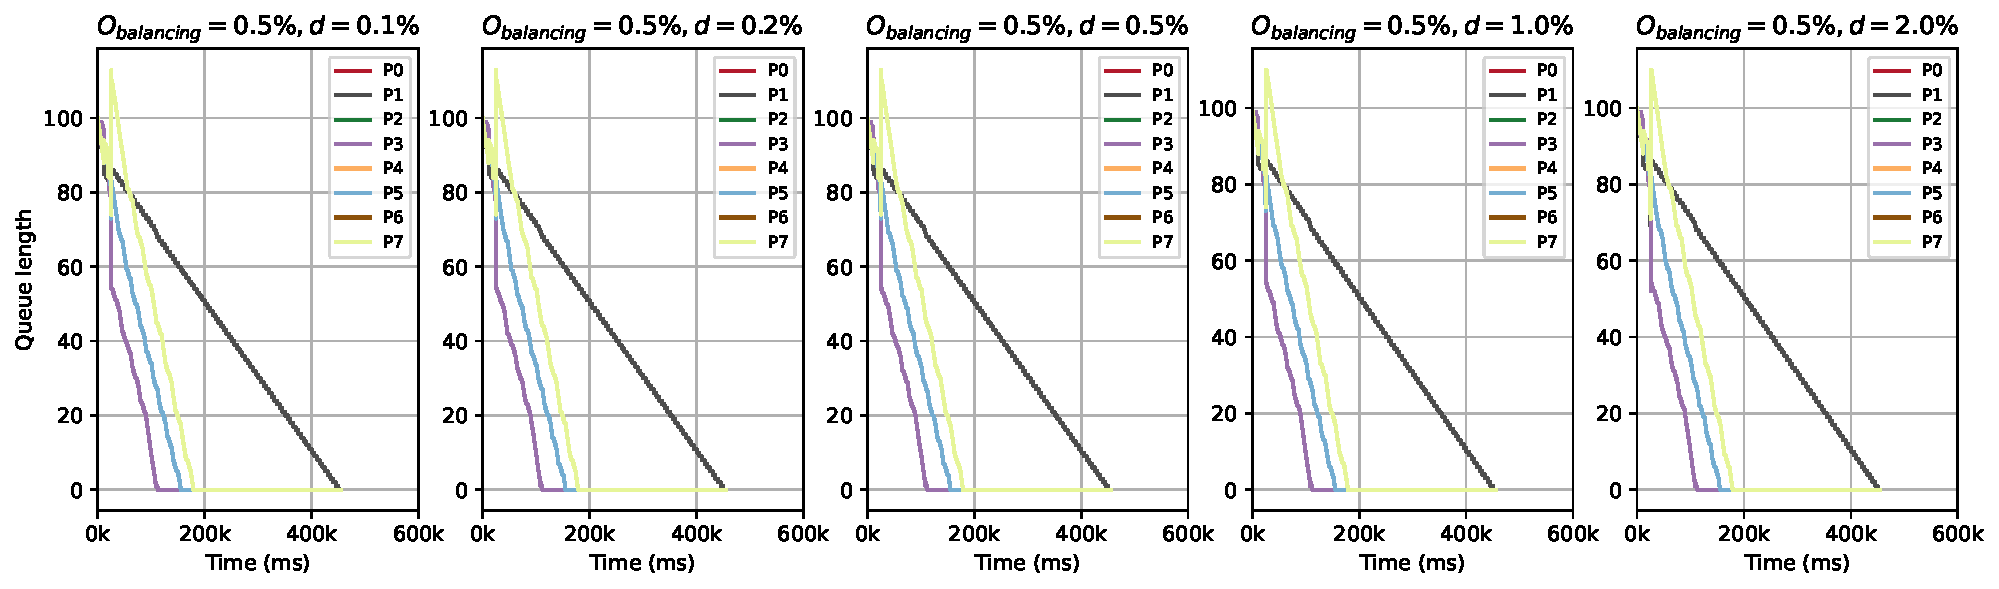
\includegraphics[scale=0.45]{./pictures/perf_analysis_model/perf_model_queue_decrease_delay_impact_OB5.pdf}
	\caption{A simulation case to show the impact of delay time ($d$) with keeping the overhead of balancing operations as a constant of $0.5\%$.}
	\label{fig:react_lb_sim_delay_impact_Obal_5}
\end{figure}

Next, we try to increase the balancing overhead a little more by $0.5\%$. Figure \ref{fig:react_lb_sim_delay_impact_Obal_5} shows the simulations with $O_{\text{balancing}}=5$. Some queues initially receive tasks from $P0$ and $P1$, for example, $P7$. This is why the $P7$ queue length is larger than $100$ tasks at that moment. In the end, the completion time is still slightly improved ($< 500$k ms) rather than the baseline. However, this simulating case shows that the overhead of balancing operations can greatly impact the time when task offloading is decided to take action. Even though the strategy of reactive load balancing can perform task migration earlier, it is still challenging during decision-making. In the next simulation scenarios, we keep $d$ as a constant and vary the value of $O_{\text{balancing}}$.\\

\noindent \textbf{Vary balancing overhead ($O_{\text{balancing}}$) and keep delay ($d$) stable}\\
\noindent In this set of simulations, we vary the values of $O_{\text{balancing}}$ in a range of $[$ $0.1\%$, $0.2\%$, $0.5\%$, $1\%$, $2\%$ $]$, and keep the values of $d$ as a constant.\\

\begin{figure}[t]
  \centering
  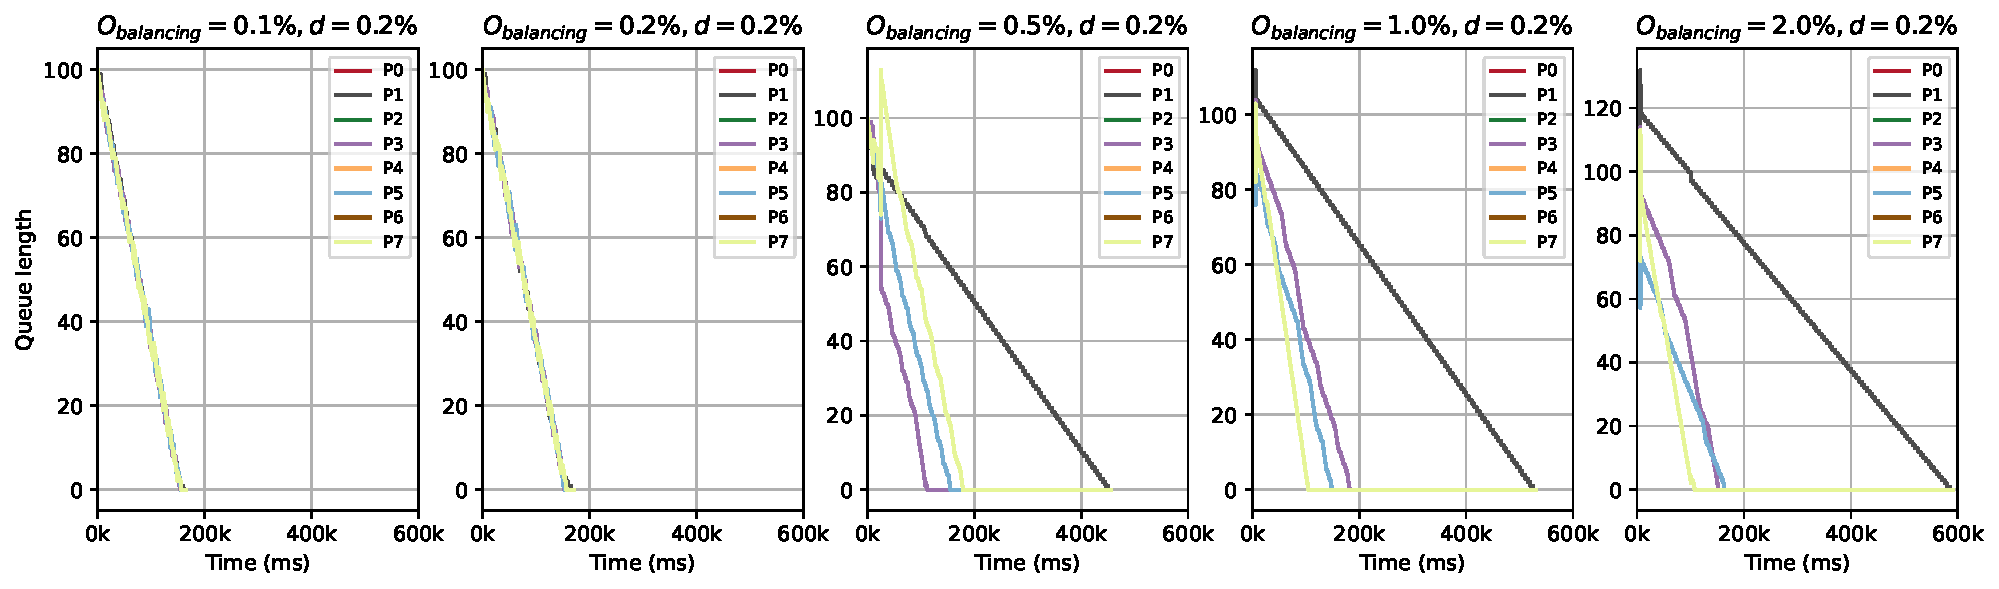
\includegraphics[scale=0.45]{./pictures/perf_analysis_model/perf_model_queue_decrease_blancing_impact_d2.pdf}
	\caption{A simulation case to show the impact of balancing-operations overhead ($O_{\text{balancing}}$) with keeping the delay time as a constant of $0.2\%$.}
	\label{fig:react_lb_sim_Obalancing_impact_d_2}
\end{figure}

Figure \ref{fig:react_lb_sim_Obalancing_impact_d_2} shows the simulation experiments with the varied values of $O_{\text{balancing}}$, while we keep $d$ as a constant of $2$ ms. As the results, the low overhead of $O_{\text{balancing}}$ is not a problem with load balancing. After $O_{\text{balancing}} \geq 0.5$, the performance get worse. In detail, the queue of $P1$ (one of the slowdown processes) converges to $0$ slow. Besides, it also get wrong task offloading. Instead of offloading tasks, it receives tasks from other processes when the offloading decision are performed incorrectly. There are two reasons for this:
\begin{itemize}
	\item Proceeding long before tasks are migrated: this means that slow processes have tried to offload as many tasks as possible at the beginning to fast processes, but it does not take immediately to proceed further for migration. Then, after a certain period, the queue of slow processes is less than the queue of fast processes, and tasks from the fast side are decided to offload to the slow side.
	\item Proceeding long before tasks are received: similar to proceed tasks for migrating, if the receiving sides proceed slowly, the tasks being on the offloading way are received late. Then, the monitored information of queues might not be correct, leading to wrong decision of task migration.
\end{itemize}

\begin{figure}[t]
  \centering
  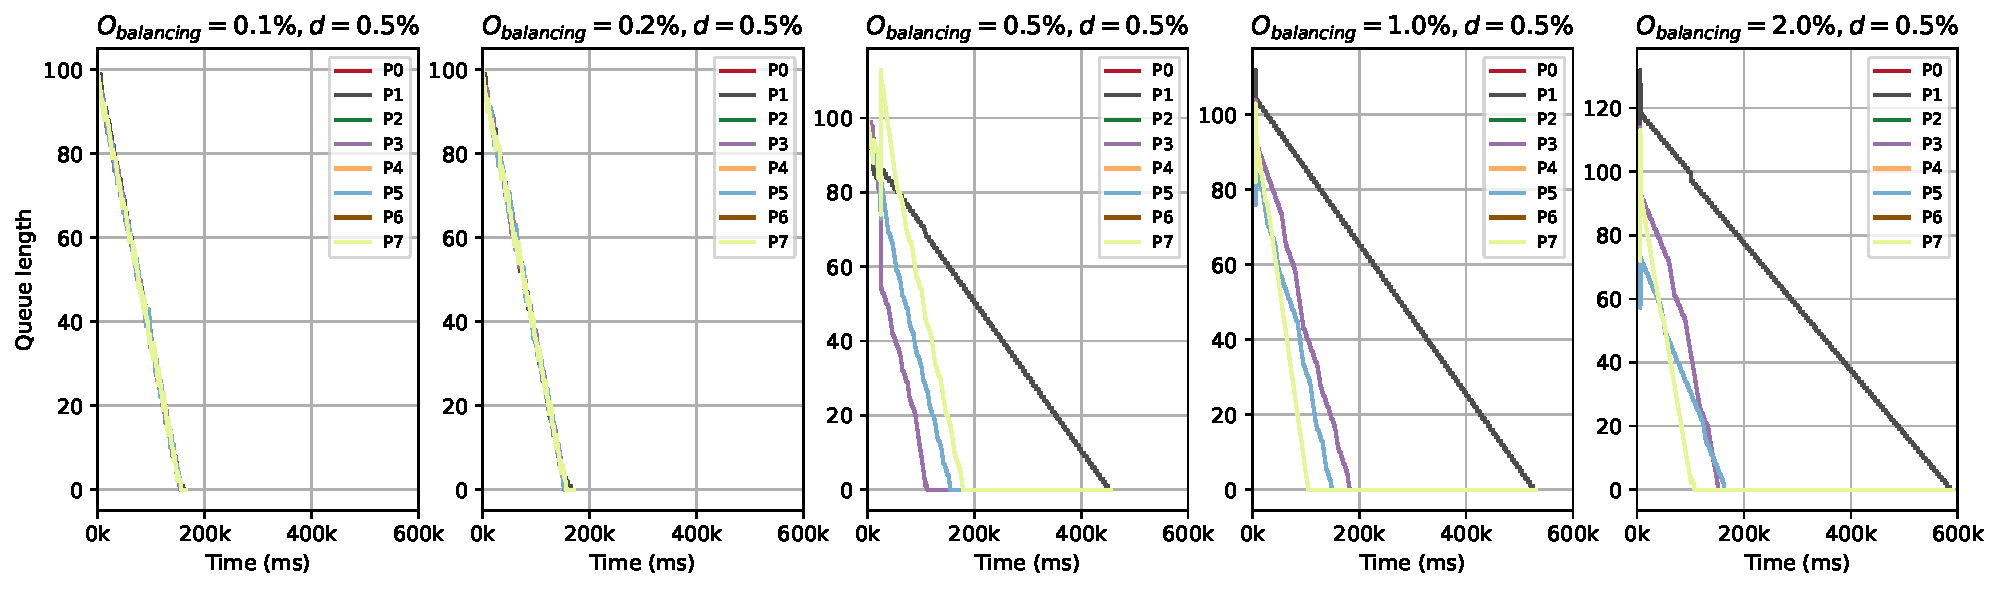
\includegraphics[scale=0.45]{./pictures/perf_analysis_model/perf_model_queue_decrease_blancing_impact_d5.pdf}
	\caption{A simulation case to show the impact of balancing-operations overhead ($O_{\text{balancing}}$) with keeping the delay time as a constant of $0.5\%$.}
	\label{fig:react_lb_sim_Obalancing_impact_d_5}
\end{figure}

Therefore, Figure \ref{fig:react_lb_sim_Obalancing_impact_d_2} reveals that the case of $O_{\text{balancing}} = 1.0$ or $O_{\text{balancing}} = 2.0$ is even worse than the baseline, even the imbalance ratio can be slightly lower but the completion time is not better. This situation is more emphasized when we continue increasing the value of $d$ to $5$ ms. Figure \ref{fig:react_lb_sim_Obalancing_impact_d_5} demonstrates the results with $d = 5$. The trend of balancing-operations impact still keeps similar.\\

\noindent \textbf{Randomize delay ($d$) and balancing overhead ($O_{\text{balancing}}$)}\\
\noindent In this set of simulations, we randomize both values of $d$ and $O_{\text{balancing}}$ in the range of $[$ $0.1\%$, $0.2\%$, ..., $5\%$ $]$. Additionally, we perform the simulations as an iterative execution. This means that we repeat the simulation over iterations. Along with the randomized values of $d$ or $O_{\text{balancing}}$, each simulation iteration can have different values of them.